\documentclass[a4paper]{article}
\usepackage[margin=1cm]{geometry}
\usepackage{amsmath, amssymb}
\usepackage{graphicx}
\usepackage{tikz}
\usetikzlibrary{arrows.meta}
\pagestyle{empty}

\definecolor{c0}{HTML}{E53935}
\definecolor{c1}{HTML}{1E88E5}
\definecolor{c2}{HTML}{43A047}
\definecolor{c3}{HTML}{FB8C00}
\definecolor{c4}{HTML}{8E24AA}
\definecolor{c5}{HTML}{00ACC1}
\definecolor{c6}{HTML}{F4511E}
\definecolor{c7}{HTML}{3949AB}
\definecolor{c8}{HTML}{7CB342}
\definecolor{c9}{HTML}{C2185B}
\definecolor{c10}{HTML}{FF7043}
\definecolor{c11}{HTML}{26A69A}
\definecolor{c12}{HTML}{5C6BC0}
\definecolor{c13}{HTML}{FFCA28}
\definecolor{c14}{HTML}{AB47BC}

\begin{document}

\begin{center}
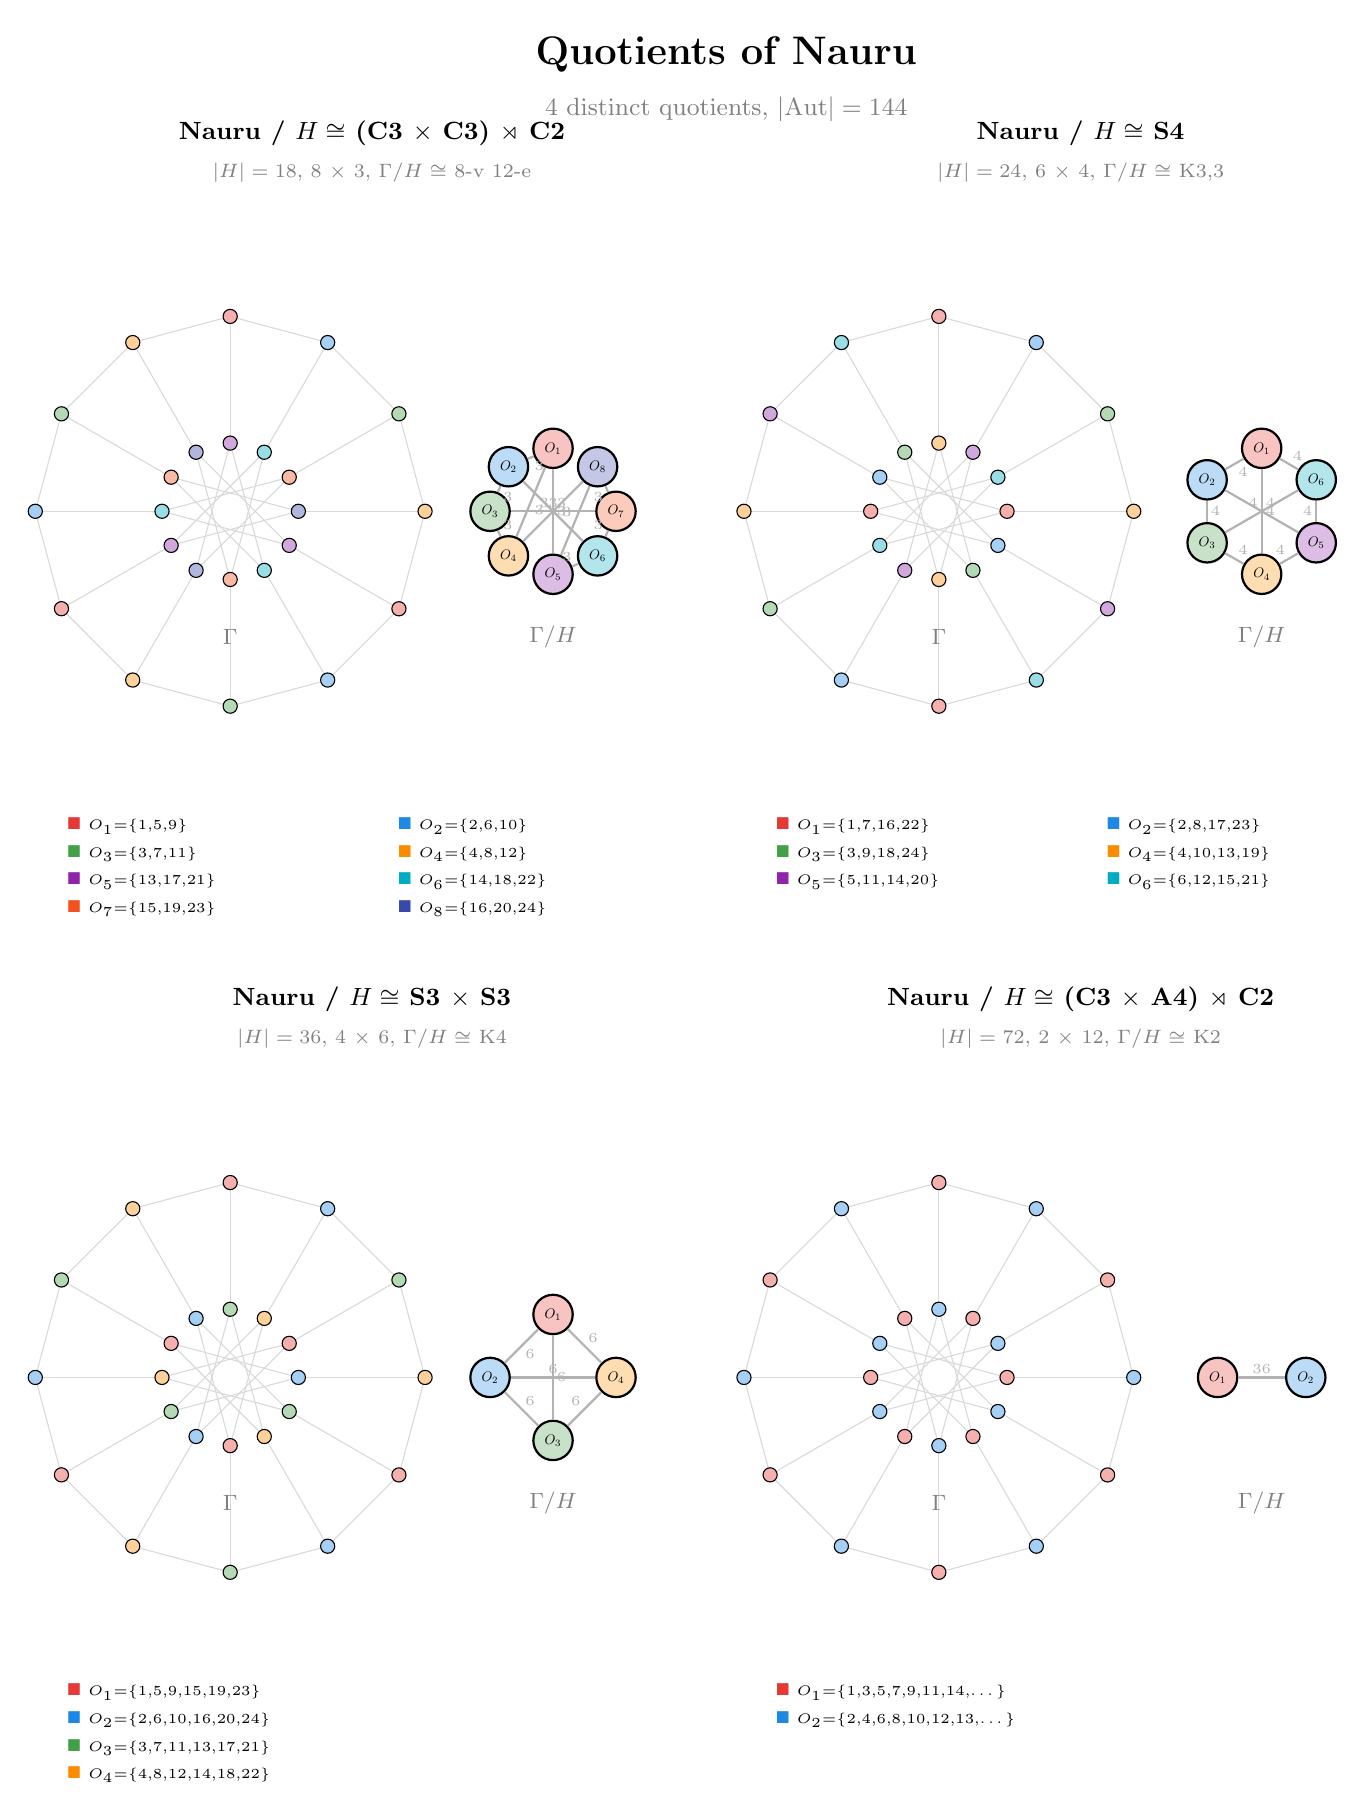
\begin{tikzpicture}[
  ov/.style={circle, draw, semithick, minimum size=3.5mm, inner sep=0pt},
  ovs/.style={circle, draw, thin, minimum size=1.8mm, inner sep=0pt},
  qv/.style={circle, draw, thick, minimum size=5mm, inner sep=0pt},
  cardtitle/.style={font=\small\bfseries},
  cardsub/.style={font=\scriptsize, text=gray},
  glabel/.style={font=\footnotesize, text=gray},
]
\node[font=\Large\bfseries] at (0, 11.5) {Quotients of Nauru};
\node[font=\small, text=gray] at (0, 10.8) {4 distinct quotients, $|\mathrm{Aut}|=144$};

% Card 1: H=(C3 x C3) : C2
\node[cardtitle] at (-4.50,10.50) {Nauru / $H \cong$ (C3 $\times$ C3) $\rtimes$ C2};
\node[cardsub] at (-4.50,10.00) {$|H|=18$, 8 $\times$ 3, $\Gamma/H \cong$ 8-v 12-e};
\draw[gray!30, thin] (-6.300,8.175) -- (-5.062,7.843);
\draw[gray!30, thin] (-6.300,8.175) -- (-7.537,7.843);
\draw[gray!30, thin] (-6.300,8.175) -- (-6.300,6.566);
\draw[gray!30, thin] (-5.062,7.843) -- (-4.157,6.938);
\draw[gray!30, thin] (-5.062,7.843) -- (-5.867,6.450);
\draw[gray!30, thin] (-4.157,6.938) -- (-3.825,5.700);
\draw[gray!30, thin] (-4.157,6.938) -- (-5.550,6.133);
\draw[gray!30, thin] (-3.825,5.700) -- (-4.157,4.462);
\draw[gray!30, thin] (-3.825,5.700) -- (-5.434,5.700);
\draw[gray!30, thin] (-4.157,4.462) -- (-5.062,3.557);
\draw[gray!30, thin] (-4.157,4.462) -- (-5.550,5.267);
\draw[gray!30, thin] (-5.062,3.557) -- (-6.300,3.225);
\draw[gray!30, thin] (-5.062,3.557) -- (-5.867,4.950);
\draw[gray!30, thin] (-6.300,3.225) -- (-7.538,3.557);
\draw[gray!30, thin] (-6.300,3.225) -- (-6.300,4.834);
\draw[gray!30, thin] (-7.538,3.557) -- (-8.443,4.463);
\draw[gray!30, thin] (-7.538,3.557) -- (-6.733,4.950);
\draw[gray!30, thin] (-8.443,4.463) -- (-8.775,5.700);
\draw[gray!30, thin] (-8.443,4.463) -- (-7.050,5.267);
\draw[gray!30, thin] (-8.775,5.700) -- (-8.443,6.938);
\draw[gray!30, thin] (-8.775,5.700) -- (-7.166,5.700);
\draw[gray!30, thin] (-8.443,6.938) -- (-7.537,7.843);
\draw[gray!30, thin] (-8.443,6.938) -- (-7.050,6.133);
\draw[gray!30, thin] (-7.537,7.843) -- (-6.733,6.450);
\draw[gray!30, thin] (-6.300,6.566) -- (-5.867,4.950);
\draw[gray!30, thin] (-6.300,6.566) -- (-6.733,4.950);
\draw[gray!30, thin] (-5.867,6.450) -- (-6.300,4.834);
\draw[gray!30, thin] (-5.867,6.450) -- (-7.050,5.267);
\draw[gray!30, thin] (-5.550,6.133) -- (-6.733,4.950);
\draw[gray!30, thin] (-5.550,6.133) -- (-7.166,5.700);
\draw[gray!30, thin] (-5.434,5.700) -- (-7.050,5.267);
\draw[gray!30, thin] (-5.434,5.700) -- (-7.050,6.133);
\draw[gray!30, thin] (-5.550,5.267) -- (-7.166,5.700);
\draw[gray!30, thin] (-5.550,5.267) -- (-6.733,6.450);
\draw[gray!30, thin] (-5.867,4.950) -- (-7.050,6.133);
\draw[gray!30, thin] (-6.300,4.834) -- (-6.733,6.450);
\node[ovs, fill=c0!40] at (-6.300,8.175) {};
\node[ovs, fill=c1!40] at (-5.062,7.843) {};
\node[ovs, fill=c2!40] at (-4.157,6.938) {};
\node[ovs, fill=c3!40] at (-3.825,5.700) {};
\node[ovs, fill=c0!40] at (-4.157,4.462) {};
\node[ovs, fill=c1!40] at (-5.062,3.557) {};
\node[ovs, fill=c2!40] at (-6.300,3.225) {};
\node[ovs, fill=c3!40] at (-7.538,3.557) {};
\node[ovs, fill=c0!40] at (-8.443,4.463) {};
\node[ovs, fill=c1!40] at (-8.775,5.700) {};
\node[ovs, fill=c2!40] at (-8.443,6.938) {};
\node[ovs, fill=c3!40] at (-7.537,7.843) {};
\node[ovs, fill=c4!40] at (-6.300,6.566) {};
\node[ovs, fill=c5!40] at (-5.867,6.450) {};
\node[ovs, fill=c6!40] at (-5.550,6.133) {};
\node[ovs, fill=c7!40] at (-5.434,5.700) {};
\node[ovs, fill=c4!40] at (-5.550,5.267) {};
\node[ovs, fill=c5!40] at (-5.867,4.950) {};
\node[ovs, fill=c6!40] at (-6.300,4.834) {};
\node[ovs, fill=c7!40] at (-6.733,4.950) {};
\node[ovs, fill=c4!40] at (-7.050,5.267) {};
\node[ovs, fill=c5!40] at (-7.166,5.700) {};
\node[ovs, fill=c6!40] at (-7.050,6.133) {};
\node[ovs, fill=c7!40] at (-6.733,6.450) {};
\node[glabel] at (-6.30,4.10) {$\Gamma$};
\node[qv, fill=c0!30] (c0o0) at (-2.200,6.500) {\scalebox{0.5}{$O_{1}$}};
\node[qv, fill=c1!30] (c0o1) at (-2.766,6.266) {\scalebox{0.5}{$O_{2}$}};
\node[qv, fill=c2!30] (c0o2) at (-3.000,5.700) {\scalebox{0.5}{$O_{3}$}};
\node[qv, fill=c3!30] (c0o3) at (-2.766,5.134) {\scalebox{0.5}{$O_{4}$}};
\node[qv, fill=c4!30] (c0o4) at (-2.200,4.900) {\scalebox{0.5}{$O_{5}$}};
\node[qv, fill=c5!30] (c0o5) at (-1.634,5.134) {\scalebox{0.5}{$O_{6}$}};
\node[qv, fill=c6!30] (c0o6) at (-1.400,5.700) {\scalebox{0.5}{$O_{7}$}};
\node[qv, fill=c7!30] (c0o7) at (-1.634,6.266) {\scalebox{0.5}{$O_{8}$}};
\draw[gray!60, thick] (c0o0) -- node[font=\tiny, auto, inner sep=1pt] {3} (c0o1);
\draw[gray!60, thick] (c0o0) -- node[font=\tiny, auto, inner sep=1pt] {3} (c0o3);
\draw[gray!60, thick] (c0o0) -- node[font=\tiny, auto, inner sep=1pt] {3} (c0o4);
\draw[gray!60, thick] (c0o1) -- node[font=\tiny, auto, inner sep=1pt] {3} (c0o2);
\draw[gray!60, thick] (c0o1) -- node[font=\tiny, auto, inner sep=1pt] {3} (c0o5);
\draw[gray!60, thick] (c0o2) -- node[font=\tiny, auto, inner sep=1pt] {3} (c0o3);
\draw[gray!60, thick] (c0o2) -- node[font=\tiny, auto, inner sep=1pt] {3} (c0o6);
\draw[gray!60, thick] (c0o3) -- node[font=\tiny, auto, inner sep=1pt] {3} (c0o7);
\draw[gray!60, thick] (c0o4) -- node[font=\tiny, auto, inner sep=1pt] {3} (c0o5);
\draw[gray!60, thick] (c0o4) -- node[font=\tiny, auto, inner sep=1pt] {3} (c0o7);
\draw[gray!60, thick] (c0o5) -- node[font=\tiny, auto, inner sep=1pt] {3} (c0o6);
\draw[gray!60, thick] (c0o6) -- node[font=\tiny, auto, inner sep=1pt] {3} (c0o7);
\node[glabel] at (-2.20,4.10) {$\Gamma/H$};
\node[anchor=west, font=\tiny] at (-8.50,1.70) {\textcolor{c0}{$\blacksquare$} $O_{1}$=\{1,5,9\}};
\node[anchor=west, font=\tiny] at (-4.30,1.70) {\textcolor{c1}{$\blacksquare$} $O_{2}$=\{2,6,10\}};
\node[anchor=west, font=\tiny] at (-8.50,1.35) {\textcolor{c2}{$\blacksquare$} $O_{3}$=\{3,7,11\}};
\node[anchor=west, font=\tiny] at (-4.30,1.35) {\textcolor{c3}{$\blacksquare$} $O_{4}$=\{4,8,12\}};
\node[anchor=west, font=\tiny] at (-8.50,1.00) {\textcolor{c4}{$\blacksquare$} $O_{5}$=\{13,17,21\}};
\node[anchor=west, font=\tiny] at (-4.30,1.00) {\textcolor{c5}{$\blacksquare$} $O_{6}$=\{14,18,22\}};
\node[anchor=west, font=\tiny] at (-8.50,0.65) {\textcolor{c6}{$\blacksquare$} $O_{7}$=\{15,19,23\}};
\node[anchor=west, font=\tiny] at (-4.30,0.65) {\textcolor{c7}{$\blacksquare$} $O_{8}$=\{16,20,24\}};

% Card 2: H=S4
\node[cardtitle] at (4.50,10.50) {Nauru / $H \cong$ S4};
\node[cardsub] at (4.50,10.00) {$|H|=24$, 6 $\times$ 4, $\Gamma/H \cong$ K3,3};
\draw[gray!30, thin] (2.700,8.175) -- (3.937,7.843);
\draw[gray!30, thin] (2.700,8.175) -- (1.463,7.843);
\draw[gray!30, thin] (2.700,8.175) -- (2.700,6.566);
\draw[gray!30, thin] (3.937,7.843) -- (4.843,6.938);
\draw[gray!30, thin] (3.937,7.843) -- (3.133,6.450);
\draw[gray!30, thin] (4.843,6.938) -- (5.175,5.700);
\draw[gray!30, thin] (4.843,6.938) -- (3.450,6.133);
\draw[gray!30, thin] (5.175,5.700) -- (4.843,4.462);
\draw[gray!30, thin] (5.175,5.700) -- (3.566,5.700);
\draw[gray!30, thin] (4.843,4.462) -- (3.938,3.557);
\draw[gray!30, thin] (4.843,4.462) -- (3.450,5.267);
\draw[gray!30, thin] (3.938,3.557) -- (2.700,3.225);
\draw[gray!30, thin] (3.938,3.557) -- (3.133,4.950);
\draw[gray!30, thin] (2.700,3.225) -- (1.462,3.557);
\draw[gray!30, thin] (2.700,3.225) -- (2.700,4.834);
\draw[gray!30, thin] (1.462,3.557) -- (0.557,4.463);
\draw[gray!30, thin] (1.462,3.557) -- (2.267,4.950);
\draw[gray!30, thin] (0.557,4.463) -- (0.225,5.700);
\draw[gray!30, thin] (0.557,4.463) -- (1.950,5.267);
\draw[gray!30, thin] (0.225,5.700) -- (0.557,6.938);
\draw[gray!30, thin] (0.225,5.700) -- (1.834,5.700);
\draw[gray!30, thin] (0.557,6.938) -- (1.463,7.843);
\draw[gray!30, thin] (0.557,6.938) -- (1.950,6.133);
\draw[gray!30, thin] (1.463,7.843) -- (2.267,6.450);
\draw[gray!30, thin] (2.700,6.566) -- (3.133,4.950);
\draw[gray!30, thin] (2.700,6.566) -- (2.267,4.950);
\draw[gray!30, thin] (3.133,6.450) -- (2.700,4.834);
\draw[gray!30, thin] (3.133,6.450) -- (1.950,5.267);
\draw[gray!30, thin] (3.450,6.133) -- (2.267,4.950);
\draw[gray!30, thin] (3.450,6.133) -- (1.834,5.700);
\draw[gray!30, thin] (3.566,5.700) -- (1.950,5.267);
\draw[gray!30, thin] (3.566,5.700) -- (1.950,6.133);
\draw[gray!30, thin] (3.450,5.267) -- (1.834,5.700);
\draw[gray!30, thin] (3.450,5.267) -- (2.267,6.450);
\draw[gray!30, thin] (3.133,4.950) -- (1.950,6.133);
\draw[gray!30, thin] (2.700,4.834) -- (2.267,6.450);
\node[ovs, fill=c0!40] at (2.700,8.175) {};
\node[ovs, fill=c1!40] at (3.937,7.843) {};
\node[ovs, fill=c2!40] at (4.843,6.938) {};
\node[ovs, fill=c3!40] at (5.175,5.700) {};
\node[ovs, fill=c4!40] at (4.843,4.462) {};
\node[ovs, fill=c5!40] at (3.938,3.557) {};
\node[ovs, fill=c0!40] at (2.700,3.225) {};
\node[ovs, fill=c1!40] at (1.462,3.557) {};
\node[ovs, fill=c2!40] at (0.557,4.463) {};
\node[ovs, fill=c3!40] at (0.225,5.700) {};
\node[ovs, fill=c4!40] at (0.557,6.938) {};
\node[ovs, fill=c5!40] at (1.463,7.843) {};
\node[ovs, fill=c3!40] at (2.700,6.566) {};
\node[ovs, fill=c4!40] at (3.133,6.450) {};
\node[ovs, fill=c5!40] at (3.450,6.133) {};
\node[ovs, fill=c0!40] at (3.566,5.700) {};
\node[ovs, fill=c1!40] at (3.450,5.267) {};
\node[ovs, fill=c2!40] at (3.133,4.950) {};
\node[ovs, fill=c3!40] at (2.700,4.834) {};
\node[ovs, fill=c4!40] at (2.267,4.950) {};
\node[ovs, fill=c5!40] at (1.950,5.267) {};
\node[ovs, fill=c0!40] at (1.834,5.700) {};
\node[ovs, fill=c1!40] at (1.950,6.133) {};
\node[ovs, fill=c2!40] at (2.267,6.450) {};
\node[glabel] at (2.70,4.10) {$\Gamma$};
\node[qv, fill=c0!30] (c1o0) at (6.800,6.500) {\scalebox{0.5}{$O_{1}$}};
\node[qv, fill=c1!30] (c1o1) at (6.107,6.100) {\scalebox{0.5}{$O_{2}$}};
\node[qv, fill=c2!30] (c1o2) at (6.107,5.300) {\scalebox{0.5}{$O_{3}$}};
\node[qv, fill=c3!30] (c1o3) at (6.800,4.900) {\scalebox{0.5}{$O_{4}$}};
\node[qv, fill=c4!30] (c1o4) at (7.493,5.300) {\scalebox{0.5}{$O_{5}$}};
\node[qv, fill=c5!30] (c1o5) at (7.493,6.100) {\scalebox{0.5}{$O_{6}$}};
\draw[gray!60, thick] (c1o0) -- node[font=\tiny, auto, inner sep=1pt] {4} (c1o1);
\draw[gray!60, thick] (c1o0) -- node[font=\tiny, auto, inner sep=1pt] {4} (c1o3);
\draw[gray!60, thick] (c1o0) -- node[font=\tiny, auto, inner sep=1pt] {4} (c1o5);
\draw[gray!60, thick] (c1o1) -- node[font=\tiny, auto, inner sep=1pt] {4} (c1o2);
\draw[gray!60, thick] (c1o1) -- node[font=\tiny, auto, inner sep=1pt] {4} (c1o4);
\draw[gray!60, thick] (c1o2) -- node[font=\tiny, auto, inner sep=1pt] {4} (c1o3);
\draw[gray!60, thick] (c1o2) -- node[font=\tiny, auto, inner sep=1pt] {4} (c1o5);
\draw[gray!60, thick] (c1o3) -- node[font=\tiny, auto, inner sep=1pt] {4} (c1o4);
\draw[gray!60, thick] (c1o4) -- node[font=\tiny, auto, inner sep=1pt] {4} (c1o5);
\node[glabel] at (6.80,4.10) {$\Gamma/H$};
\node[anchor=west, font=\tiny] at (0.50,1.70) {\textcolor{c0}{$\blacksquare$} $O_{1}$=\{1,7,16,22\}};
\node[anchor=west, font=\tiny] at (4.70,1.70) {\textcolor{c1}{$\blacksquare$} $O_{2}$=\{2,8,17,23\}};
\node[anchor=west, font=\tiny] at (0.50,1.35) {\textcolor{c2}{$\blacksquare$} $O_{3}$=\{3,9,18,24\}};
\node[anchor=west, font=\tiny] at (4.70,1.35) {\textcolor{c3}{$\blacksquare$} $O_{4}$=\{4,10,13,19\}};
\node[anchor=west, font=\tiny] at (0.50,1.00) {\textcolor{c4}{$\blacksquare$} $O_{5}$=\{5,11,14,20\}};
\node[anchor=west, font=\tiny] at (4.70,1.00) {\textcolor{c5}{$\blacksquare$} $O_{6}$=\{6,12,15,21\}};

% Card 3: H=S3 x S3
\node[cardtitle] at (-4.50,-0.50) {Nauru / $H \cong$ S3 $\times$ S3};
\node[cardsub] at (-4.50,-1.00) {$|H|=36$, 4 $\times$ 6, $\Gamma/H \cong$ K4};
\draw[gray!30, thin] (-6.300,-2.825) -- (-5.062,-3.157);
\draw[gray!30, thin] (-6.300,-2.825) -- (-7.537,-3.157);
\draw[gray!30, thin] (-6.300,-2.825) -- (-6.300,-4.434);
\draw[gray!30, thin] (-5.062,-3.157) -- (-4.157,-4.062);
\draw[gray!30, thin] (-5.062,-3.157) -- (-5.867,-4.550);
\draw[gray!30, thin] (-4.157,-4.062) -- (-3.825,-5.300);
\draw[gray!30, thin] (-4.157,-4.062) -- (-5.550,-4.867);
\draw[gray!30, thin] (-3.825,-5.300) -- (-4.157,-6.538);
\draw[gray!30, thin] (-3.825,-5.300) -- (-5.434,-5.300);
\draw[gray!30, thin] (-4.157,-6.538) -- (-5.062,-7.443);
\draw[gray!30, thin] (-4.157,-6.538) -- (-5.550,-5.733);
\draw[gray!30, thin] (-5.062,-7.443) -- (-6.300,-7.775);
\draw[gray!30, thin] (-5.062,-7.443) -- (-5.867,-6.050);
\draw[gray!30, thin] (-6.300,-7.775) -- (-7.538,-7.443);
\draw[gray!30, thin] (-6.300,-7.775) -- (-6.300,-6.166);
\draw[gray!30, thin] (-7.538,-7.443) -- (-8.443,-6.537);
\draw[gray!30, thin] (-7.538,-7.443) -- (-6.733,-6.050);
\draw[gray!30, thin] (-8.443,-6.537) -- (-8.775,-5.300);
\draw[gray!30, thin] (-8.443,-6.537) -- (-7.050,-5.733);
\draw[gray!30, thin] (-8.775,-5.300) -- (-8.443,-4.062);
\draw[gray!30, thin] (-8.775,-5.300) -- (-7.166,-5.300);
\draw[gray!30, thin] (-8.443,-4.062) -- (-7.537,-3.157);
\draw[gray!30, thin] (-8.443,-4.062) -- (-7.050,-4.867);
\draw[gray!30, thin] (-7.537,-3.157) -- (-6.733,-4.550);
\draw[gray!30, thin] (-6.300,-4.434) -- (-5.867,-6.050);
\draw[gray!30, thin] (-6.300,-4.434) -- (-6.733,-6.050);
\draw[gray!30, thin] (-5.867,-4.550) -- (-6.300,-6.166);
\draw[gray!30, thin] (-5.867,-4.550) -- (-7.050,-5.733);
\draw[gray!30, thin] (-5.550,-4.867) -- (-6.733,-6.050);
\draw[gray!30, thin] (-5.550,-4.867) -- (-7.166,-5.300);
\draw[gray!30, thin] (-5.434,-5.300) -- (-7.050,-5.733);
\draw[gray!30, thin] (-5.434,-5.300) -- (-7.050,-4.867);
\draw[gray!30, thin] (-5.550,-5.733) -- (-7.166,-5.300);
\draw[gray!30, thin] (-5.550,-5.733) -- (-6.733,-4.550);
\draw[gray!30, thin] (-5.867,-6.050) -- (-7.050,-4.867);
\draw[gray!30, thin] (-6.300,-6.166) -- (-6.733,-4.550);
\node[ovs, fill=c0!40] at (-6.300,-2.825) {};
\node[ovs, fill=c1!40] at (-5.062,-3.157) {};
\node[ovs, fill=c2!40] at (-4.157,-4.062) {};
\node[ovs, fill=c3!40] at (-3.825,-5.300) {};
\node[ovs, fill=c0!40] at (-4.157,-6.538) {};
\node[ovs, fill=c1!40] at (-5.062,-7.443) {};
\node[ovs, fill=c2!40] at (-6.300,-7.775) {};
\node[ovs, fill=c3!40] at (-7.538,-7.443) {};
\node[ovs, fill=c0!40] at (-8.443,-6.537) {};
\node[ovs, fill=c1!40] at (-8.775,-5.300) {};
\node[ovs, fill=c2!40] at (-8.443,-4.062) {};
\node[ovs, fill=c3!40] at (-7.537,-3.157) {};
\node[ovs, fill=c2!40] at (-6.300,-4.434) {};
\node[ovs, fill=c3!40] at (-5.867,-4.550) {};
\node[ovs, fill=c0!40] at (-5.550,-4.867) {};
\node[ovs, fill=c1!40] at (-5.434,-5.300) {};
\node[ovs, fill=c2!40] at (-5.550,-5.733) {};
\node[ovs, fill=c3!40] at (-5.867,-6.050) {};
\node[ovs, fill=c0!40] at (-6.300,-6.166) {};
\node[ovs, fill=c1!40] at (-6.733,-6.050) {};
\node[ovs, fill=c2!40] at (-7.050,-5.733) {};
\node[ovs, fill=c3!40] at (-7.166,-5.300) {};
\node[ovs, fill=c0!40] at (-7.050,-4.867) {};
\node[ovs, fill=c1!40] at (-6.733,-4.550) {};
\node[glabel] at (-6.30,-6.90) {$\Gamma$};
\node[qv, fill=c0!30] (c2o0) at (-2.200,-4.500) {\scalebox{0.5}{$O_{1}$}};
\node[qv, fill=c1!30] (c2o1) at (-3.000,-5.300) {\scalebox{0.5}{$O_{2}$}};
\node[qv, fill=c2!30] (c2o2) at (-2.200,-6.100) {\scalebox{0.5}{$O_{3}$}};
\node[qv, fill=c3!30] (c2o3) at (-1.400,-5.300) {\scalebox{0.5}{$O_{4}$}};
\draw[gray!60, thick] (c2o0) -- node[font=\tiny, auto, inner sep=1pt] {6} (c2o1);
\draw[gray!60, thick] (c2o0) -- node[font=\tiny, auto, inner sep=1pt] {6} (c2o2);
\draw[gray!60, thick] (c2o0) -- node[font=\tiny, auto, inner sep=1pt] {6} (c2o3);
\draw[gray!60, thick] (c2o1) -- node[font=\tiny, auto, inner sep=1pt] {6} (c2o2);
\draw[gray!60, thick] (c2o1) -- node[font=\tiny, auto, inner sep=1pt] {6} (c2o3);
\draw[gray!60, thick] (c2o2) -- node[font=\tiny, auto, inner sep=1pt] {6} (c2o3);
\node[glabel] at (-2.20,-6.90) {$\Gamma/H$};
\node[anchor=west, font=\tiny] at (-8.50,-9.30) {\textcolor{c0}{$\blacksquare$} $O_{1}$=\{1,5,9,15,19,23\}};
\node[anchor=west, font=\tiny] at (-8.50,-9.65) {\textcolor{c1}{$\blacksquare$} $O_{2}$=\{2,6,10,16,20,24\}};
\node[anchor=west, font=\tiny] at (-8.50,-10.00) {\textcolor{c2}{$\blacksquare$} $O_{3}$=\{3,7,11,13,17,21\}};
\node[anchor=west, font=\tiny] at (-8.50,-10.35) {\textcolor{c3}{$\blacksquare$} $O_{4}$=\{4,8,12,14,18,22\}};

% Card 4: H=(C3 x A4) : C2
\node[cardtitle] at (4.50,-0.50) {Nauru / $H \cong$ (C3 $\times$ A4) $\rtimes$ C2};
\node[cardsub] at (4.50,-1.00) {$|H|=72$, 2 $\times$ 12, $\Gamma/H \cong$ K2};
\draw[gray!30, thin] (2.700,-2.825) -- (3.937,-3.157);
\draw[gray!30, thin] (2.700,-2.825) -- (1.463,-3.157);
\draw[gray!30, thin] (2.700,-2.825) -- (2.700,-4.434);
\draw[gray!30, thin] (3.937,-3.157) -- (4.843,-4.062);
\draw[gray!30, thin] (3.937,-3.157) -- (3.133,-4.550);
\draw[gray!30, thin] (4.843,-4.062) -- (5.175,-5.300);
\draw[gray!30, thin] (4.843,-4.062) -- (3.450,-4.867);
\draw[gray!30, thin] (5.175,-5.300) -- (4.843,-6.538);
\draw[gray!30, thin] (5.175,-5.300) -- (3.566,-5.300);
\draw[gray!30, thin] (4.843,-6.538) -- (3.938,-7.443);
\draw[gray!30, thin] (4.843,-6.538) -- (3.450,-5.733);
\draw[gray!30, thin] (3.938,-7.443) -- (2.700,-7.775);
\draw[gray!30, thin] (3.938,-7.443) -- (3.133,-6.050);
\draw[gray!30, thin] (2.700,-7.775) -- (1.462,-7.443);
\draw[gray!30, thin] (2.700,-7.775) -- (2.700,-6.166);
\draw[gray!30, thin] (1.462,-7.443) -- (0.557,-6.537);
\draw[gray!30, thin] (1.462,-7.443) -- (2.267,-6.050);
\draw[gray!30, thin] (0.557,-6.537) -- (0.225,-5.300);
\draw[gray!30, thin] (0.557,-6.537) -- (1.950,-5.733);
\draw[gray!30, thin] (0.225,-5.300) -- (0.557,-4.062);
\draw[gray!30, thin] (0.225,-5.300) -- (1.834,-5.300);
\draw[gray!30, thin] (0.557,-4.062) -- (1.463,-3.157);
\draw[gray!30, thin] (0.557,-4.062) -- (1.950,-4.867);
\draw[gray!30, thin] (1.463,-3.157) -- (2.267,-4.550);
\draw[gray!30, thin] (2.700,-4.434) -- (3.133,-6.050);
\draw[gray!30, thin] (2.700,-4.434) -- (2.267,-6.050);
\draw[gray!30, thin] (3.133,-4.550) -- (2.700,-6.166);
\draw[gray!30, thin] (3.133,-4.550) -- (1.950,-5.733);
\draw[gray!30, thin] (3.450,-4.867) -- (2.267,-6.050);
\draw[gray!30, thin] (3.450,-4.867) -- (1.834,-5.300);
\draw[gray!30, thin] (3.566,-5.300) -- (1.950,-5.733);
\draw[gray!30, thin] (3.566,-5.300) -- (1.950,-4.867);
\draw[gray!30, thin] (3.450,-5.733) -- (1.834,-5.300);
\draw[gray!30, thin] (3.450,-5.733) -- (2.267,-4.550);
\draw[gray!30, thin] (3.133,-6.050) -- (1.950,-4.867);
\draw[gray!30, thin] (2.700,-6.166) -- (2.267,-4.550);
\node[ovs, fill=c0!40] at (2.700,-2.825) {};
\node[ovs, fill=c1!40] at (3.937,-3.157) {};
\node[ovs, fill=c0!40] at (4.843,-4.062) {};
\node[ovs, fill=c1!40] at (5.175,-5.300) {};
\node[ovs, fill=c0!40] at (4.843,-6.538) {};
\node[ovs, fill=c1!40] at (3.938,-7.443) {};
\node[ovs, fill=c0!40] at (2.700,-7.775) {};
\node[ovs, fill=c1!40] at (1.462,-7.443) {};
\node[ovs, fill=c0!40] at (0.557,-6.537) {};
\node[ovs, fill=c1!40] at (0.225,-5.300) {};
\node[ovs, fill=c0!40] at (0.557,-4.062) {};
\node[ovs, fill=c1!40] at (1.463,-3.157) {};
\node[ovs, fill=c1!40] at (2.700,-4.434) {};
\node[ovs, fill=c0!40] at (3.133,-4.550) {};
\node[ovs, fill=c1!40] at (3.450,-4.867) {};
\node[ovs, fill=c0!40] at (3.566,-5.300) {};
\node[ovs, fill=c1!40] at (3.450,-5.733) {};
\node[ovs, fill=c0!40] at (3.133,-6.050) {};
\node[ovs, fill=c1!40] at (2.700,-6.166) {};
\node[ovs, fill=c0!40] at (2.267,-6.050) {};
\node[ovs, fill=c1!40] at (1.950,-5.733) {};
\node[ovs, fill=c0!40] at (1.834,-5.300) {};
\node[ovs, fill=c1!40] at (1.950,-4.867) {};
\node[ovs, fill=c0!40] at (2.267,-4.550) {};
\node[glabel] at (2.70,-6.90) {$\Gamma$};
\node[qv, fill=c0!30] (c3o0) at (6.240,-5.300) {\scalebox{0.5}{$O_{1}$}};
\node[qv, fill=c1!30] (c3o1) at (7.360,-5.300) {\scalebox{0.5}{$O_{2}$}};
\draw[gray!60, thick] (c3o0) -- node[font=\tiny, auto, inner sep=1pt] {36} (c3o1);
\node[glabel] at (6.80,-6.90) {$\Gamma/H$};
\node[anchor=west, font=\tiny] at (0.50,-9.30) {\textcolor{c0}{$\blacksquare$} $O_{1}$=\{1,3,5,7,9,11,14,\ldots\}};
\node[anchor=west, font=\tiny] at (0.50,-9.65) {\textcolor{c1}{$\blacksquare$} $O_{2}$=\{2,4,6,8,10,12,13,\ldots\}};
\end{tikzpicture}
\end{center}

\end{document}